% Copyright (C) The IMR developers. SPDX-License-Identifier: GPL-3.0-or-later
\documentclass[tikz,border=8pt]{standalone}
\usepackage[T1]{fontenc}
\usepackage{lmodern}
\usetikzlibrary{arrows.meta,calc}
\definecolor{ink}{HTML}{122D4A}
\definecolor{wave}{HTML}{2776C9}
\definecolor{heat}{HTML}{DF8D32}
\definecolor{rheo}{HTML}{168B88}
\begin{document}
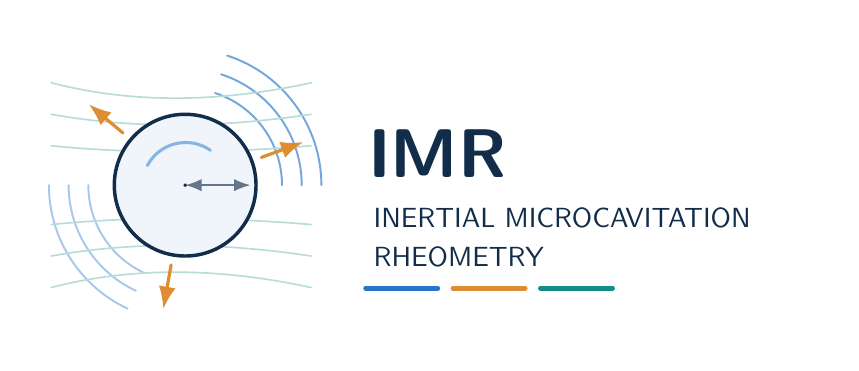
\begin{tikzpicture}[>=Latex,font=\sffamily,line cap=round,line join=round]
  \fill[white] (-2,-2) rectangle (8.2,2);
  \foreach \r in {1.23,1.48,1.73} {
    \draw[wave!65,line width=.7pt] (\r,0) arc[start angle=0,end angle=72,radius=\r];
    \draw[wave!40,line width=.7pt] (-\r,0) arc[start angle=180,end angle=245,radius=\r];
  }
  \foreach \y in {-1.3,-.9,-.5,.5,.9,1.3}
    \draw[rheo!30,line width=.6pt] (-1.7,\y) .. controls (-.7,\y*.8) and (.4,\y*.8) .. (1.6,\y);
  \fill[wave!7] (0,0) circle (.9);
  \draw[ink,line width=1.25pt] (0,0) circle (.9);
  \draw[wave!55,line width=1.1pt] (-.48,.25) arc[start angle=152,end angle=55,radius=.55];
  \foreach \a in {20,140,260} {
    \draw[->,heat,line width=1.15pt] (\a:1.03) -- (\a:1.6);
  }
  \draw[<->,ink!65,line width=.65pt] (0,0) -- (.83,0);
  \fill[ink] (0,0) circle (.025);
  \node[anchor=west,text=ink,font=\sffamily\bfseries\fontsize{49}{52}\selectfont] at (2.2,.4) {IMR};
  \node[anchor=west,text=ink,font=\sffamily\fontsize{10}{14}\selectfont,align=left] at (2.27,-.66)
    {INERTIAL MICROCAVITATION\\RHEOMETRY};
  \draw[wave,line width=1.6pt] (2.29,-1.31) -- (3.21,-1.31);
  \draw[heat,line width=1.6pt] (3.4,-1.31) -- (4.32,-1.31);
  \draw[rheo,line width=1.6pt] (4.51,-1.31) -- (5.43,-1.31);
\end{tikzpicture}
\end{document}
